\setcounter{page}{2}

\section{Задание №1}

Проект представляет собой разработку программного приложения для автоматизации деятельности небольшой коммерческой компании.
В проекте участвуют 8 разработчиков, бюджет проекта~---~не более 620 тыс. рублей, длительность проекта~---~не более 4 месяцев.
Дата начала проекта~---~первый понедельник второго квартала текущего года рабочий день марта текущего года (07.04.25).

Перед добавлением задач необходимо настроить параметры проекта, находящиеся во вкладке $\text{Файл} \rightarrow \text{Параметры} \rightarrow \text{Расписание}$.
Настройка параметров представлена на рисунке~\ref{fig:parameters}.

\begin{figure}[H]
	\centering
	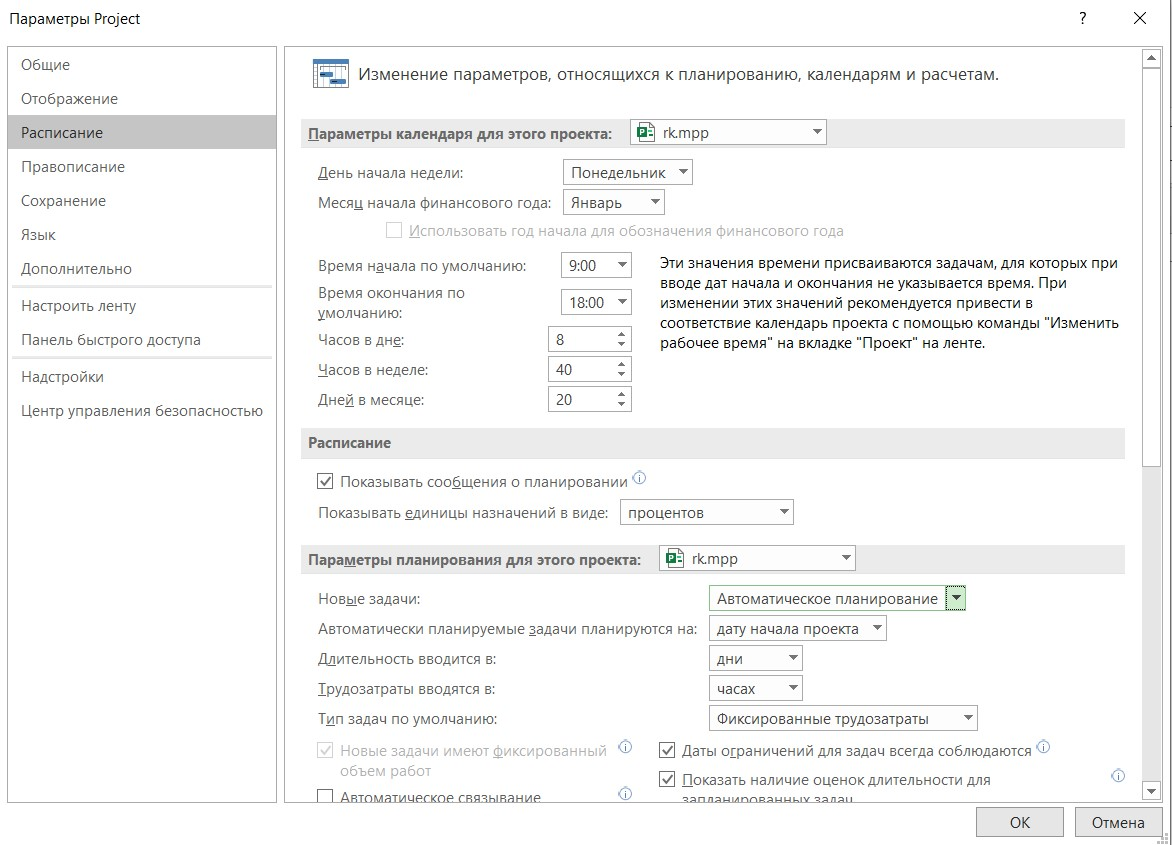
\includegraphics[width=0.9\textwidth]{img/task1/screen1_1.jpg}
	\caption{Настройка параметров проекта}
	\label{fig:parameters}
\end{figure}

Также необходимо внести в календарь праздничные дни и предшествующие им дни с укороченным рабочим графиком.
Для планируемого проекта такими днями являются майские праздники и день России.
Настройка календаря проекта приведена на рисунках~\ref{fig:calendar} и~\ref{fig:day}.

\begin{figure}[H]
	\centering
	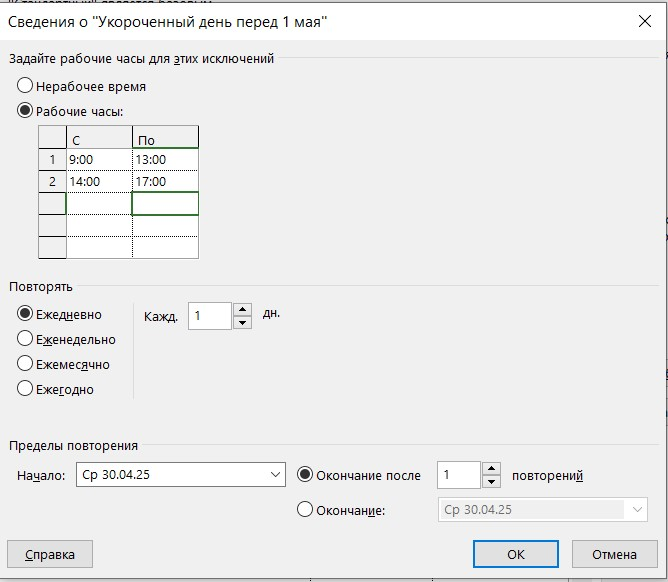
\includegraphics[width=0.9\textwidth]{img/task1/screen1_2.jpg}
	\caption{Настройка календаря проекта}
	\label{fig:calendar}
\end{figure}

\begin{figure}[H]
	\centering
	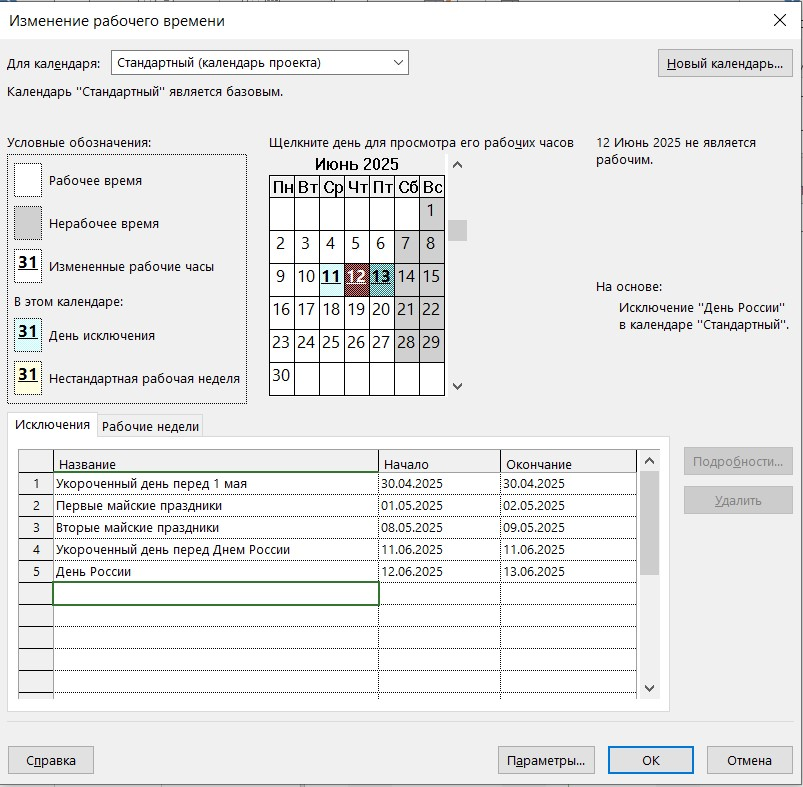
\includegraphics[width=0.9\textwidth]{img/task1/screen1_3.jpg}
	\caption{Настройка укороченного дня}
	\label{fig:day}
\end{figure}

Настройка даты начала проекта приведена на рисунке~\ref{fig:sum}.

\begin{figure}[H]
	\centering
	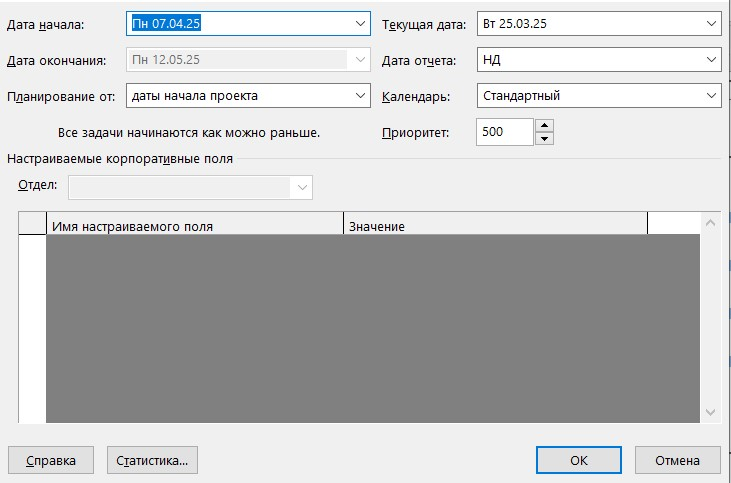
\includegraphics[width=0.9\textwidth]{img/task1/screen1_4.jpg}
	\caption{Настройка даты начала проекта}
	\label{fig:sum}
\end{figure}

Для суммарной задачи проекта указана количественная информация в заметках.
Суммарная задача приведена на рисунке~\ref{fig:notes}.

\begin{figure}[H]
	\centering
	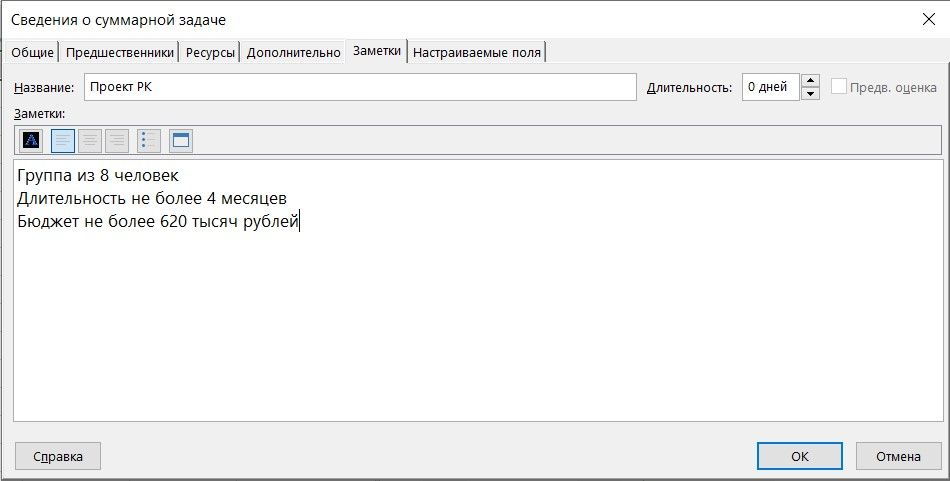
\includegraphics[width=0.9\textwidth]{img/task1/screen1_5.jpg}
	\caption{Заметки суммарной задачи}
	\label{fig:notes}
\end{figure}


\section{Задание №2}

После настройки параметров проекта необходимо добавить задачи.
Так как в настройках указано, что автоматически планируемые задачи планируются на дату начала проекта, все задачи начинаются с 07.04, что видно столбцу <<Начало>> на рисунках~\ref{fig:task2} и~\ref{fig:task2_1}.

\begin{figure}[H]
	\centering
	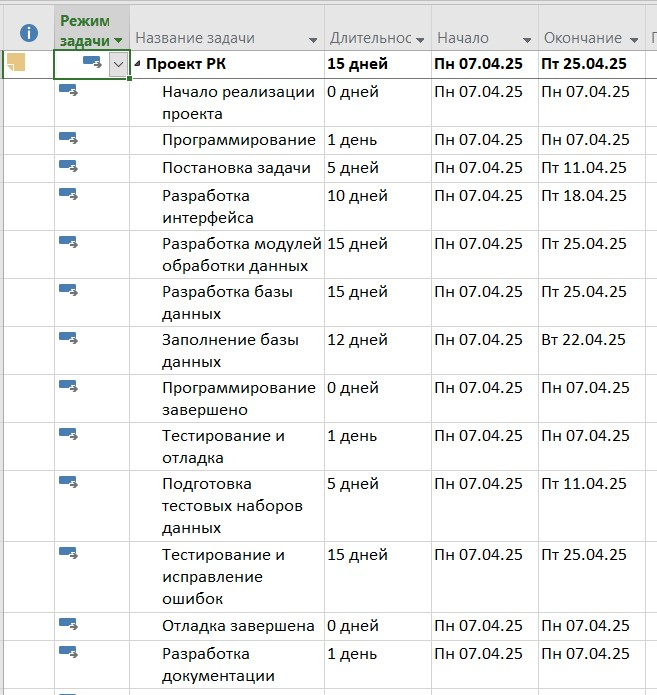
\includegraphics[width=0.9\textwidth]{img/task2/screen2_1.jpg}
	\caption{Задачи проекта}
	\label{fig:task2}
\end{figure}

\begin{figure}[H]
	\centering
	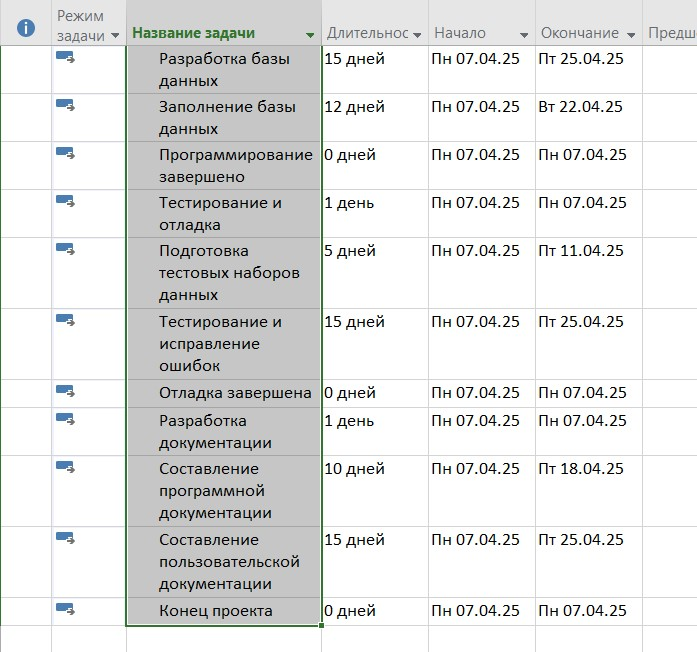
\includegraphics[width=0.9\textwidth]{img/task2/screen2_2.jpg}
	\caption{Задачи проекта}
	\label{fig:task2_1}
\end{figure}

\section{Задание №3}

При проведении структурирования списка задач были выделены фазы проекта.
Результат структурирования списка задач приведен на рисунке~\ref{fig:task3}.

\begin{figure}[H]
	\centering
	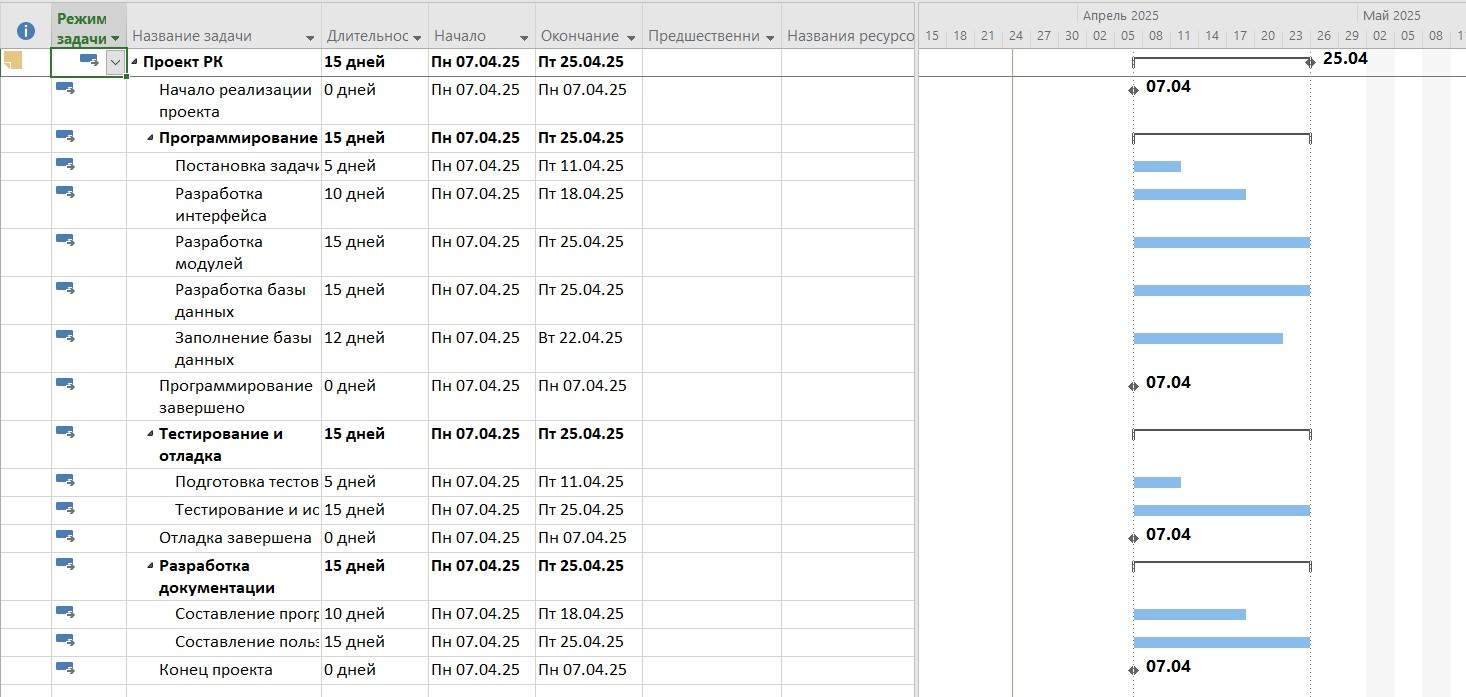
\includegraphics[width=0.9\textwidth]{img/task3/task3.jpg}
	\caption{Диаграмма Ганта после структурирования списка задач}
	\label{fig:task3}
\end{figure}

\section{Задание №4}

Задание связей между задачами приведено на рисунке~\ref{fig:task4_1}.

\begin{figure}[H]
	\centering
	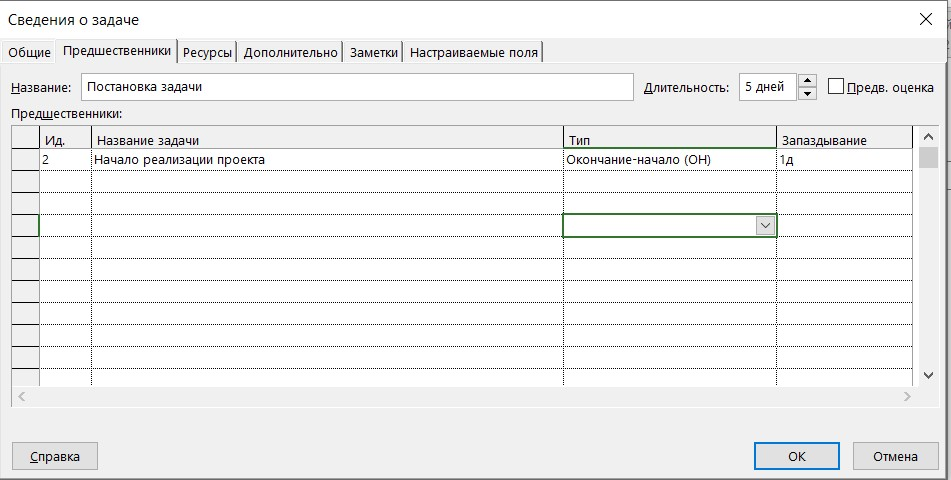
\includegraphics[width=0.9\textwidth]{img/task4/screen4_1.jpg}
	\caption{Диаграмма Ганта после структурирования списка задач}
	\label{fig:task4_1}
\end{figure}

В результате планирования проекта было определена дата завершения проекта: 18 июля 2025 года.
Таким образом, проект уложился в срок 4 месяца.

\section{Задание №5}

Лист ресурсов приведен на рисунке~\ref{fig:list}.

\begin{figure}[H]
	\centering
	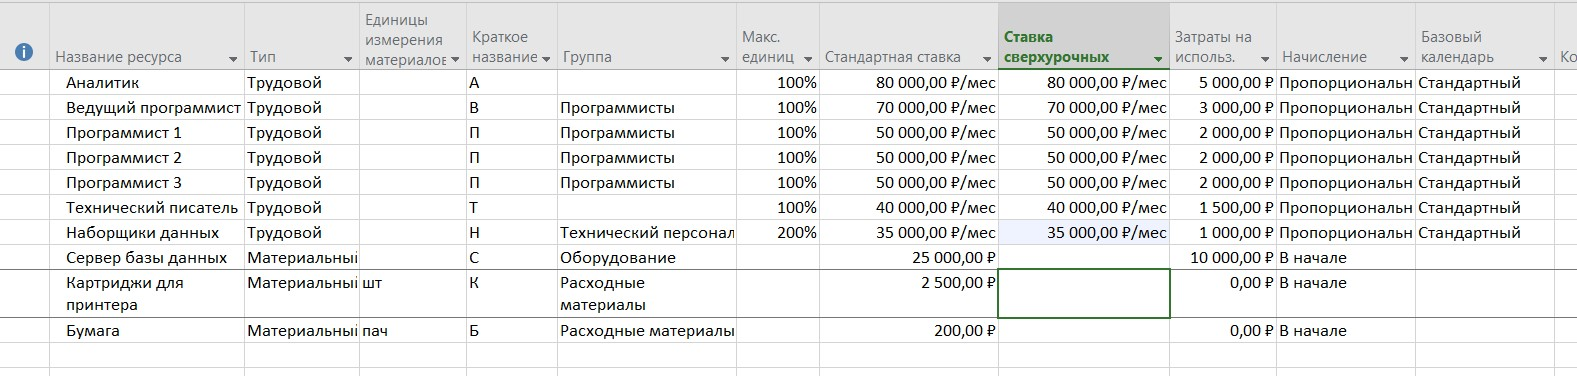
\includegraphics[width=0.9\textwidth]{img/task5/screen5_1.jpg}
	\caption{Лист ресурсов}
	\label{fig:list}
\end{figure}

\section{Задание №6}

Назначение ресурса на задачу приведено на рисунке~\ref{fig:resourse}.

\begin{figure}[H]
	\centering
	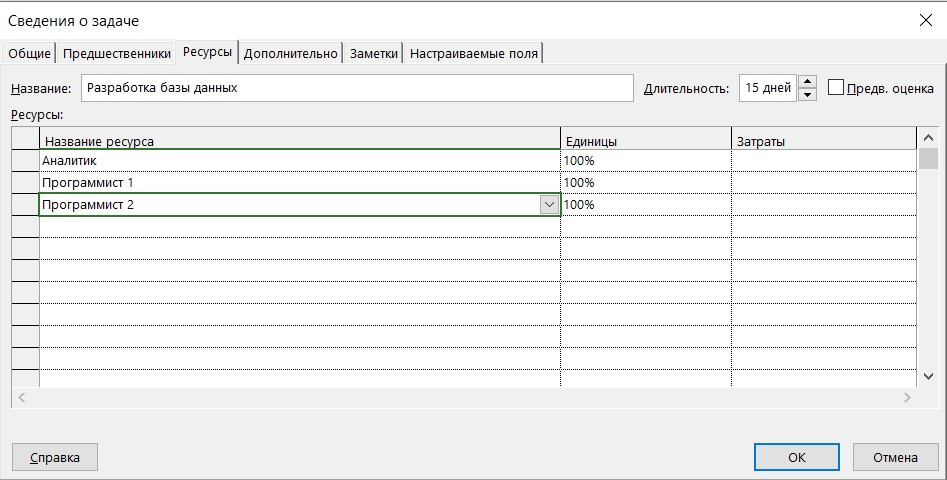
\includegraphics[width=0.9\textwidth]{img/task6/screen6_1.jpg}
	\caption{Назначение ресурса на задачу}
	\label{fig:resourse}
\end{figure}

Назначение расхода бумаги и картриджей приведено на рисунке~\ref{fig:paper}.

\begin{figure}[H]
	\centering
	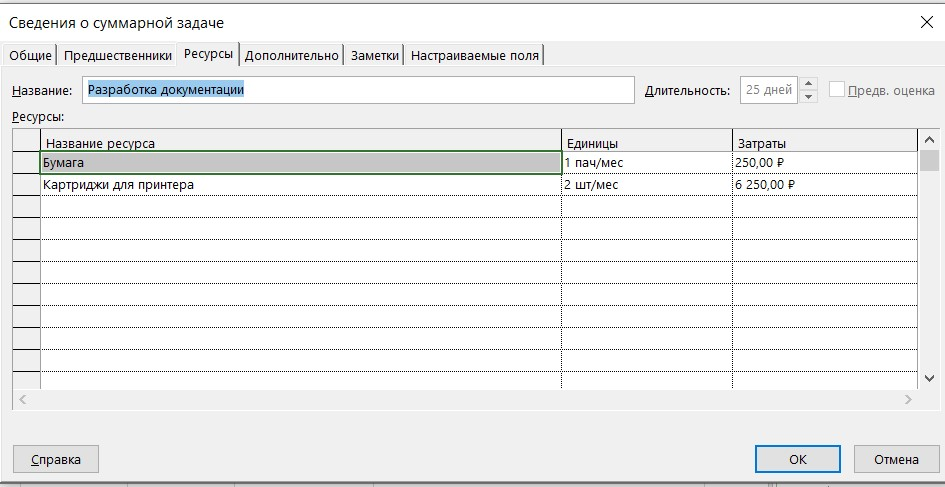
\includegraphics[width=0.9\textwidth]{img/task6/screen6_3.jpg}
	\caption{Назначение расхода бумаги}
	\label{fig:paper}
\end{figure}

\begin{figure}[H]
	\centering
	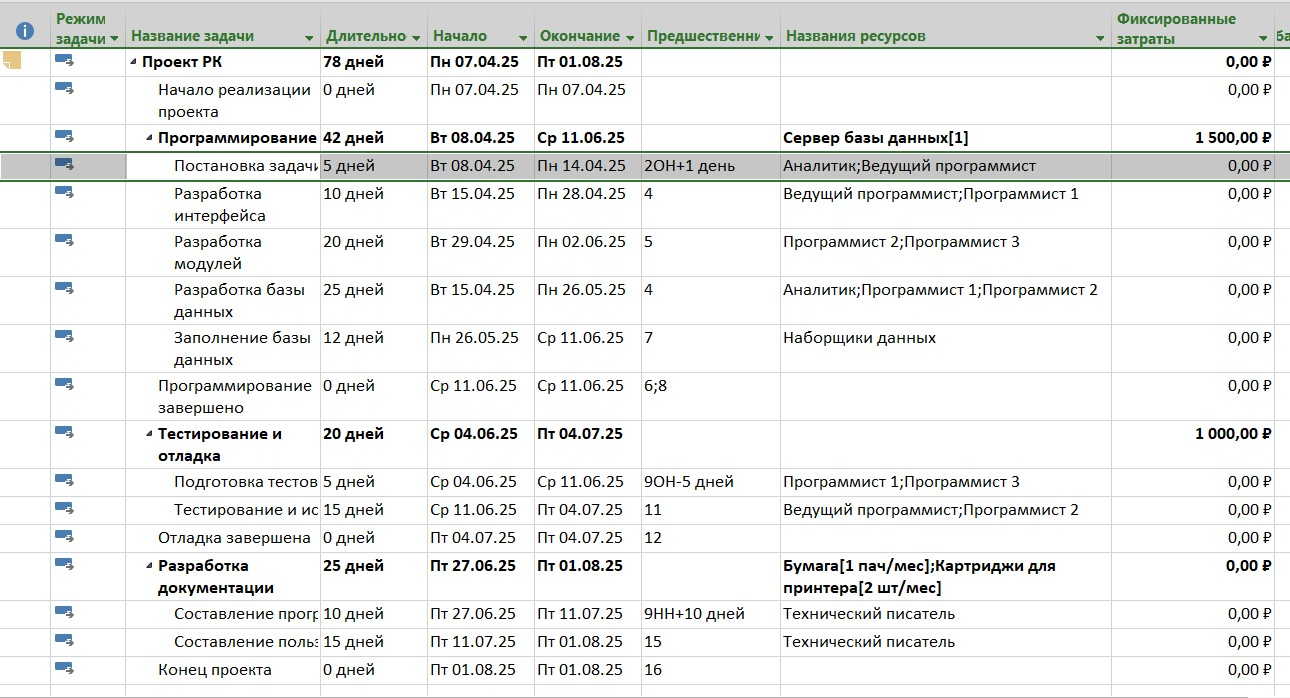
\includegraphics[width=0.9\textwidth]{img/task6/screen6_4.jpg}
	\caption{Диаграмма Ганта после усатновки на расход бумаги}
	\label{fig:paper1}
\end{figure}

\section{Задание №7}

Возникновение перегрузок показано на рисунках~\ref{fig:screen7_1} и~\ref{fig:screen7_2}.

\begin{figure}[H]
	\centering
	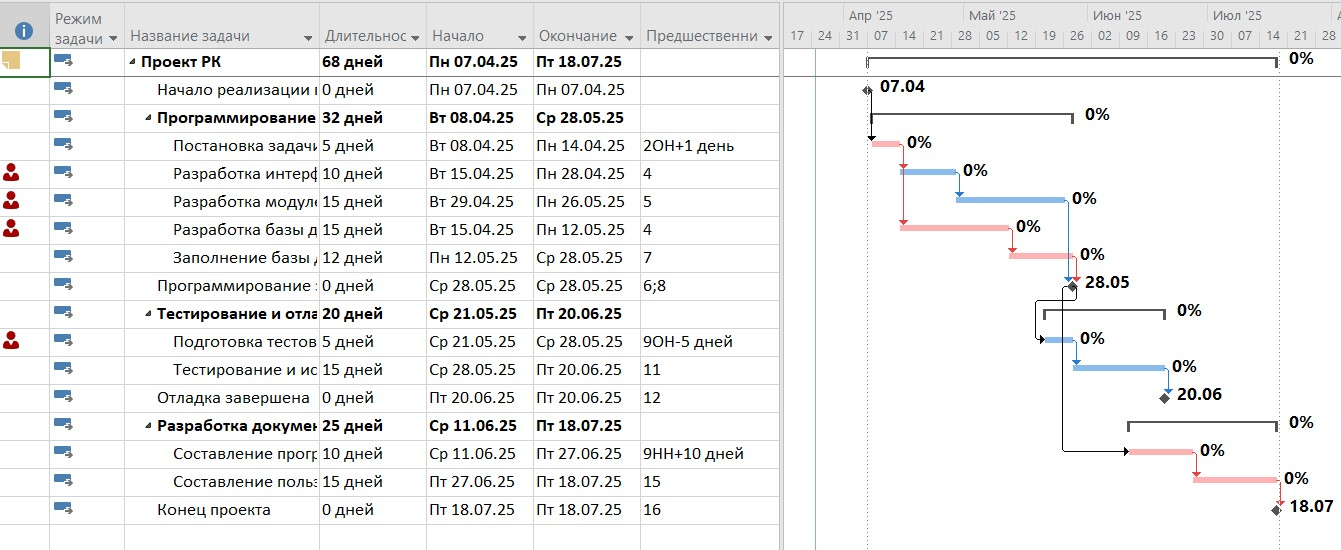
\includegraphics[width=0.9\textwidth]{img/task7/screen7_3.jpg}
	\caption{Возникновение перегрузок на диаграмме Ганта}
	\label{fig:screen7_1}
\end{figure}

\begin{figure}[H]
	\centering
	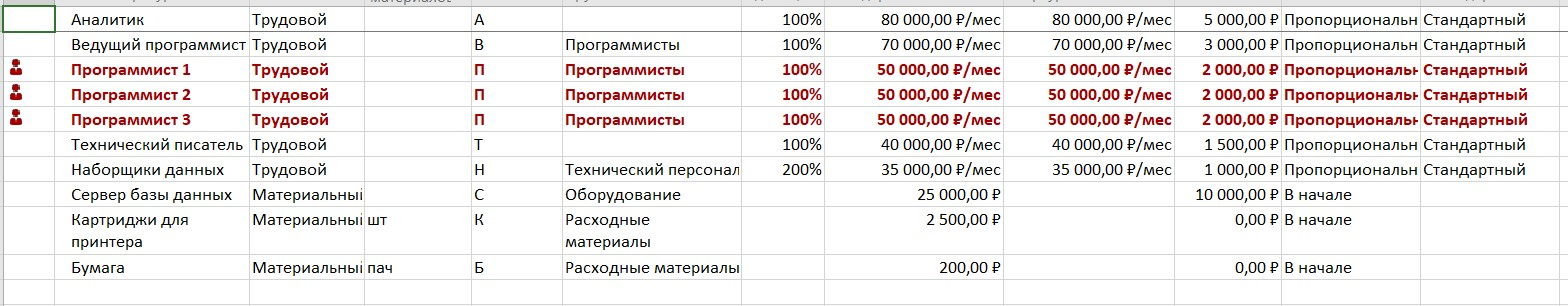
\includegraphics[width=0.9\textwidth]{img/task7/screen7_2.jpg}
	\caption{Возникновение перегрузок в листе ресурсов}
	\label{fig:screen7_2}
\end{figure}

Перегрузки возникают из-за того, что у первого программиста перекрываются задачи <<Разработка интерфейса>> и <<Разработка базы данных>>, для второго программиста перекрываются задачи <<Разработка базы данных>> и <<Разработка модулей>>, для третьего программиста~---~<<Разработка модулей>> и <<Подготовка тестов>>.
В задачу разработки базы данных невозможно добавить задержки, так как она входит в критический путь.

Устранение перегрузок демонстируется на рисунке~\ref{fig:screen7_3}.

\begin{figure}[H]
	\centering
	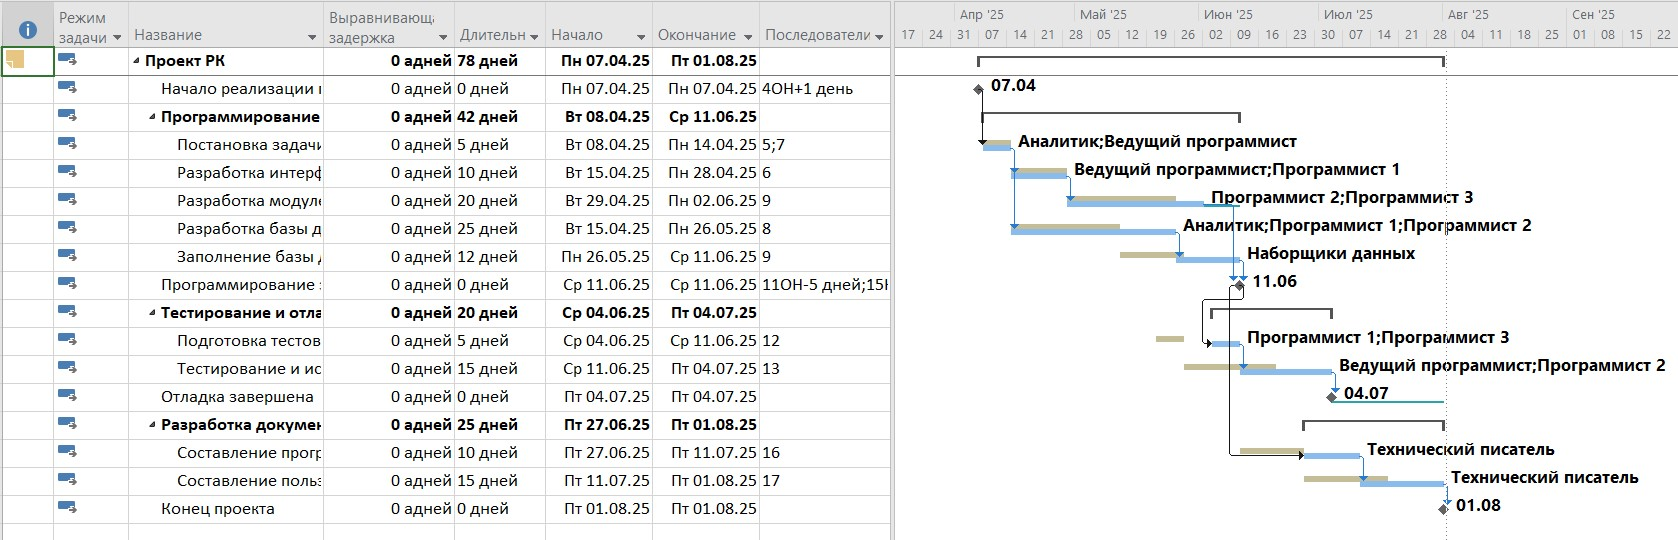
\includegraphics[width=0.9\textwidth]{img/task7/screen7_4.jpg}
	\caption{Устранение перегрузок}
	\label{fig:screen7_3}
\end{figure}

Как видно, увеличился срок задач <<Разработка базы данных>> и <<Разработка модулей>> (25 дней вместо 15 дней, 20 дней вместо 15), из-за чего были сдвинуты даты задач набора данных, тестирования и написания документации.
Дата окончания проекта изменилась с 18.07 на 01.08.

\section{Задание №8}

Добавление повторяющейся задачи профилактики показано на рисунке~\ref{fig:screen8_1}.

\begin{figure}[H]
	\centering
	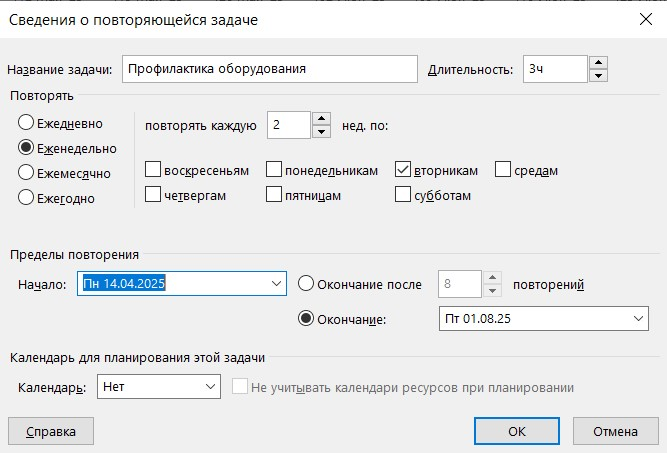
\includegraphics[width=0.9\textwidth]{img/task8/screen8_1.jpg}
	\caption{Параметры повторяющейся задачи}
	\label{fig:screen8_1}
\end{figure}

Для всех кроме специалиста по профилактике необходимо ввести перерыв в работе на время профилактики, а для профилактики создать отдельный календарь на основе стандартного, что показано на рисунках~\ref{fig:screen8_5} и~\ref{fig:screen8_6}.

\begin{figure}[H]
	\centering
	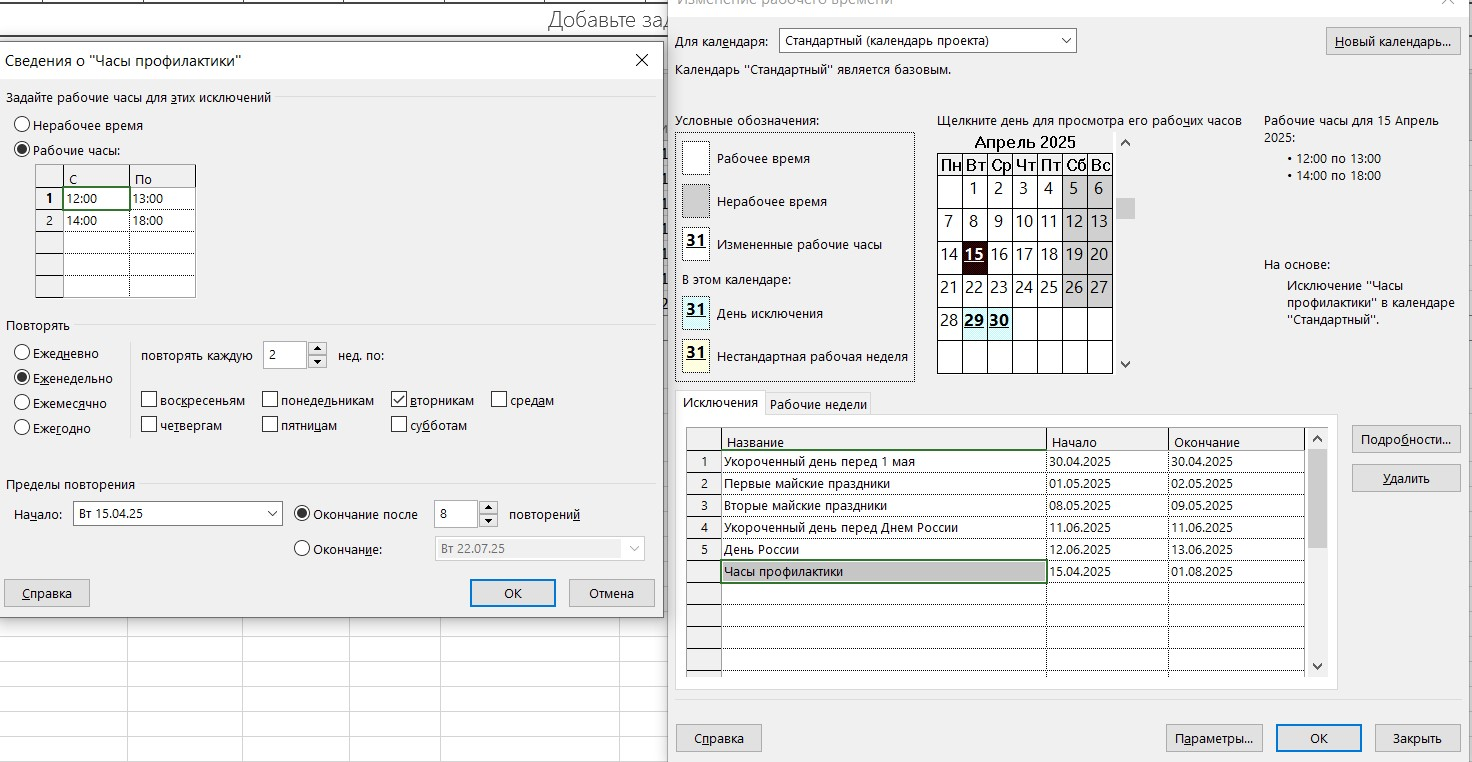
\includegraphics[width=0.9\textwidth]{img/task8/screen8_5.jpg}
	\caption{Ввод часов для профилактики}
	\label{fig:screen8_5}
\end{figure}

\begin{figure}[H]
	\centering
	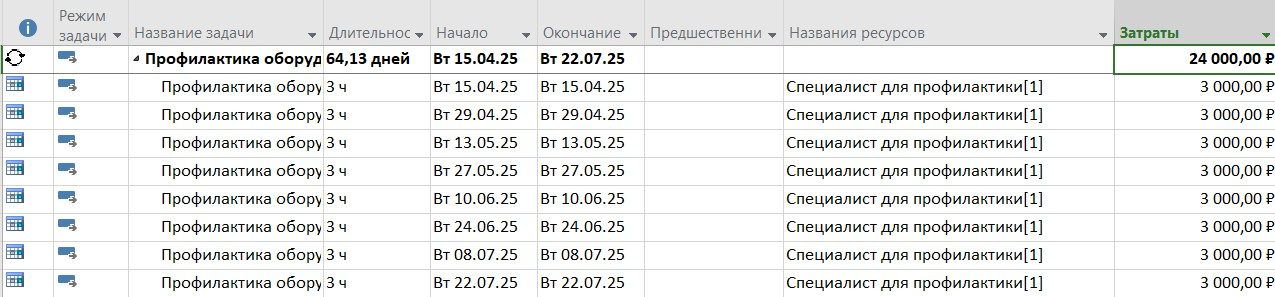
\includegraphics[width=0.9\textwidth]{img/task8/screen8_4.jpg}
	\caption{Календарь для специалиста по профилактике}
	\label{fig:screen8_6}
\end{figure}

После введения профилактики дата окончания проекта сместилась на 06.08, затраты на профилактику составили 270000 рублей, что показано на рисунке~\ref{fig:screen8_7}.

\begin{figure}[H]
	\centering
	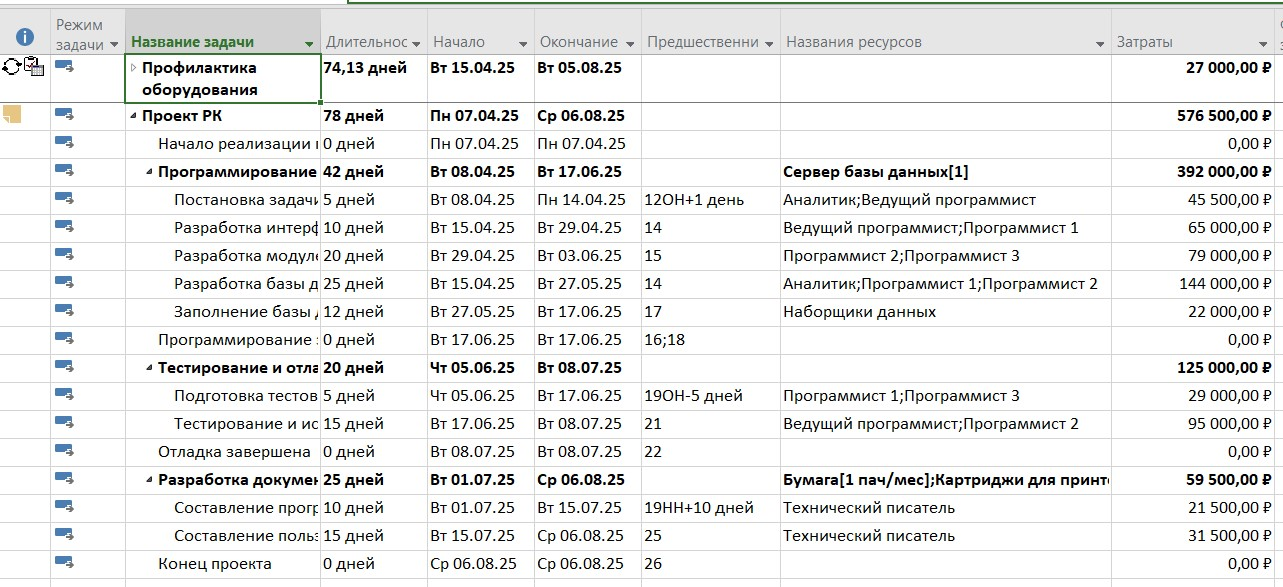
\includegraphics[width=0.9\textwidth]{img/task8/screen8_7.jpg}
	\caption{Сроки проекта после введения профилактики}
	\label{fig:screen8_7}
\end{figure}

\section{Задание №9}

Критический путь показан на рисунке~\ref{fig:screen9_0}.

\begin{figure}[H]
	\centering
	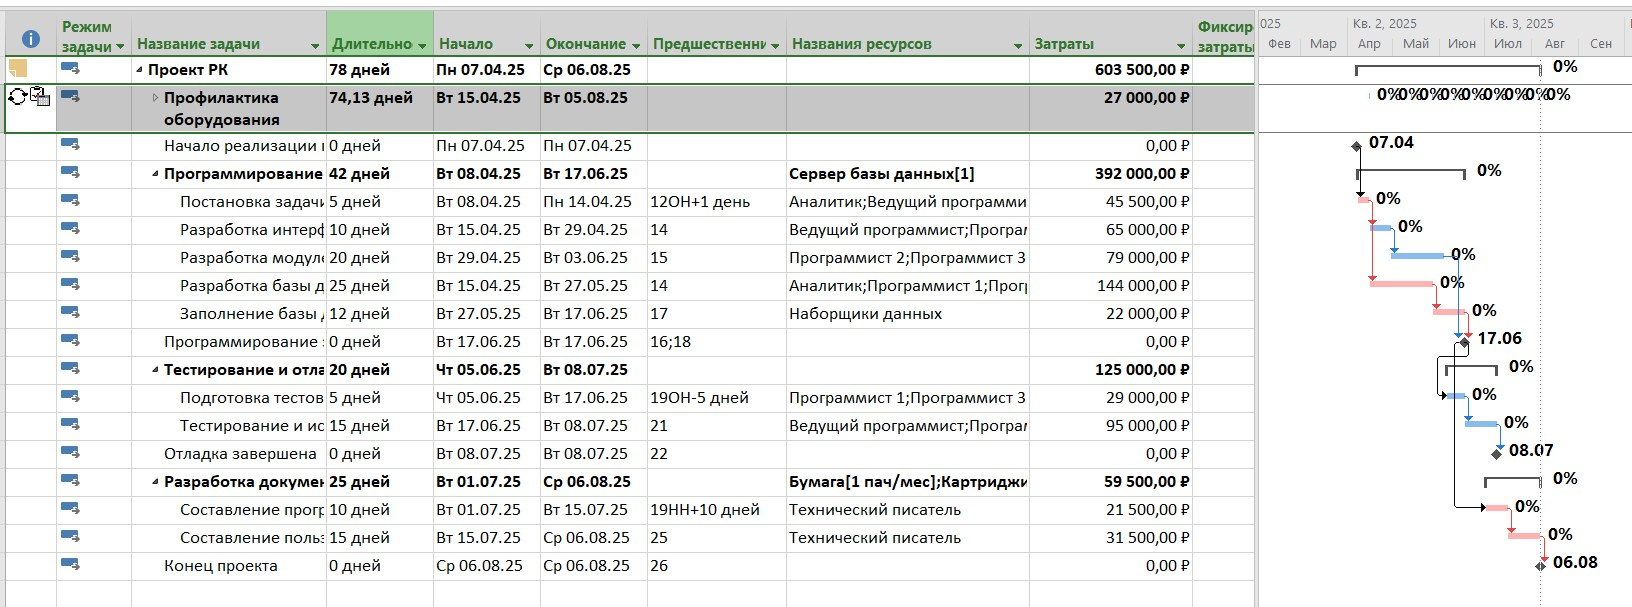
\includegraphics[width=0.9\textwidth]{img/task9/screen9_0.jpg}
	\caption{Параметры до оптимизации критического пути}
	\label{fig:screen9_0}
\end{figure}

До оптимизации критического пути проект заканчивался 06.08, затраты составили 603500 рублей.

Для оптимизации критического пути на задачу разработки базы данных был добавлен программист №3, так как он в это время почти не задействован в других задачах.

Диаграмма Ганта после оптимизации критического пути приведена на рисунке~\ref{fig:screen9_1}.

\begin{figure}[H]
	\centering
	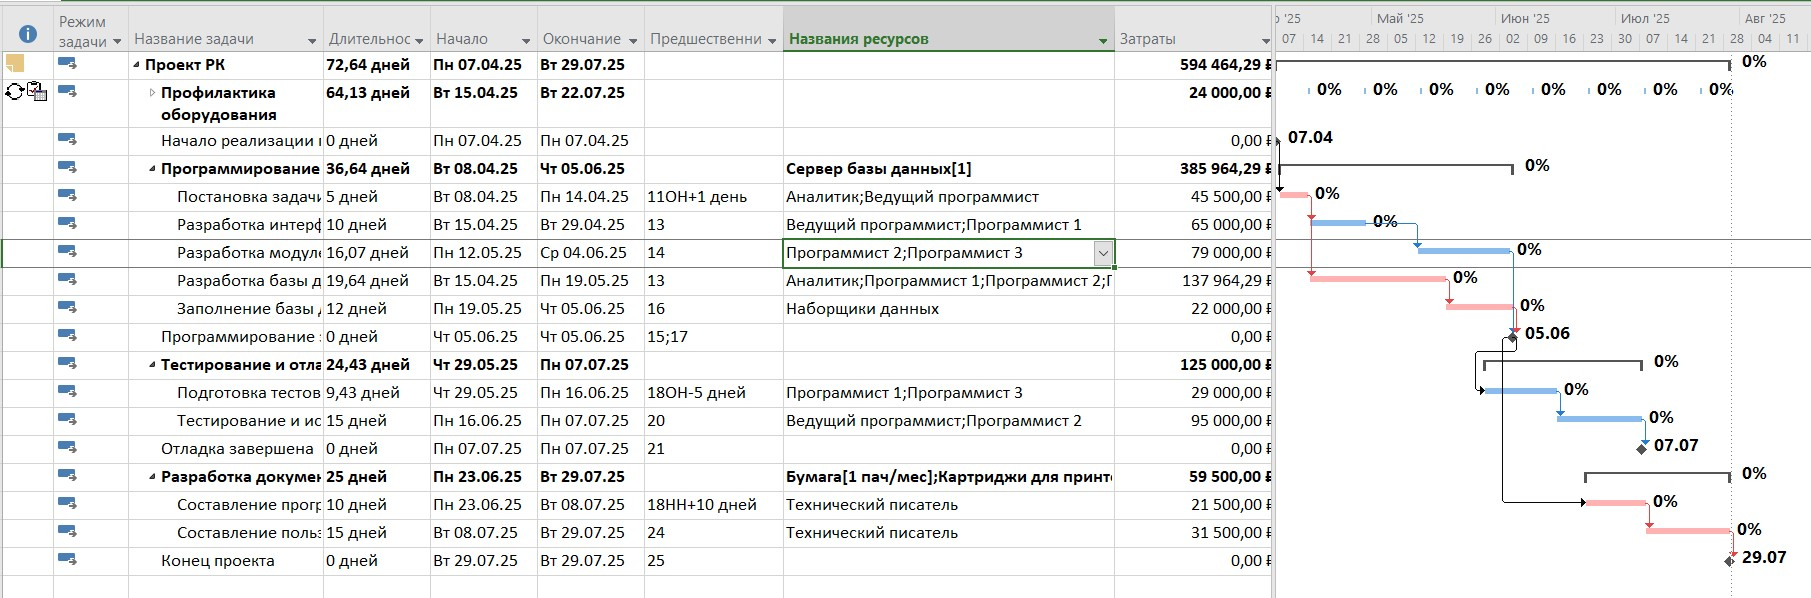
\includegraphics[width=0.9\textwidth]{img/task9/screen9_1.jpg}
	\caption{Параметры после оптимизации критического пути}
	\label{fig:screen9_1}
\end{figure}

Дата окончания проекта стала 29.07, затраты снизились до 594464 рублей, что укладывается в бюджет проекта, но не укладывается в сроки.

Задание базового плана приведено на рисунке~\ref{fig:screen9_2}.

\begin{figure}[H]
	\centering
	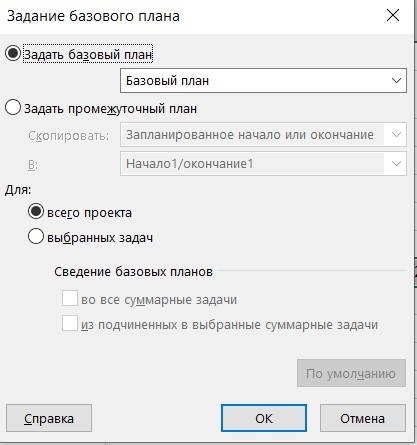
\includegraphics[width=0.9\textwidth]{img/task9/screen9_3.jpg}
	\caption{Задание базового плана}
	\label{fig:screen9_2}
\end{figure}

\section{Задание №10}

Дата отчета установлена на 09.06, что показано на рисунке~\ref{fig:screen10_1}.

\begin{figure}[H]
	\centering
	
\includegraphics[width=0.9\textwidth]{img/task10/screen10_1.jpg}
	\caption{Задание даты отчета}
	\label{fig:screen10_1}
\end{figure}

С 07.05 программисты 1 и 3 стали получать на 10\% больше, их ставка составила 550000 рублей в месяц.

\begin{figure}[H]
	\centering
	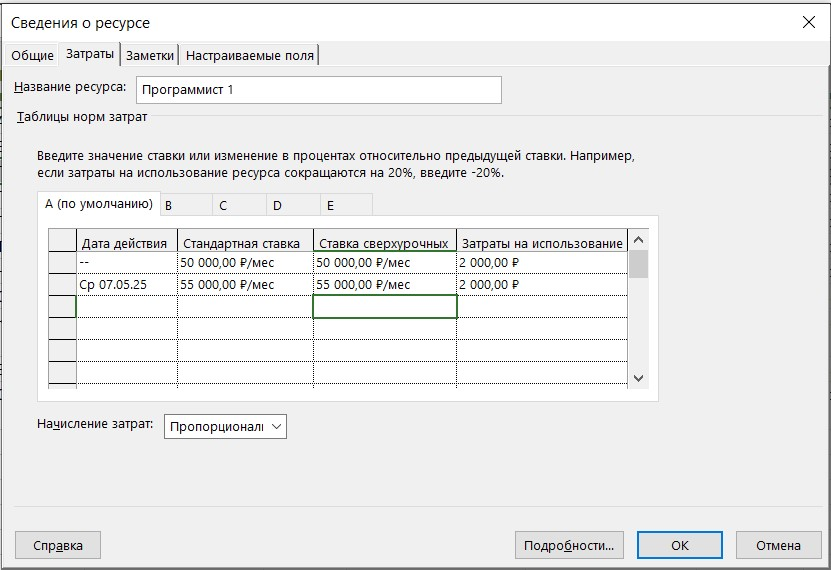
\includegraphics[width=0.9\textwidth]{img/task10/screen10_3.jpg}
	\caption{Обновление ставки программиста №1}
	\label{fig:screen10_3}
\end{figure}

\begin{figure}[H]
	\centering
	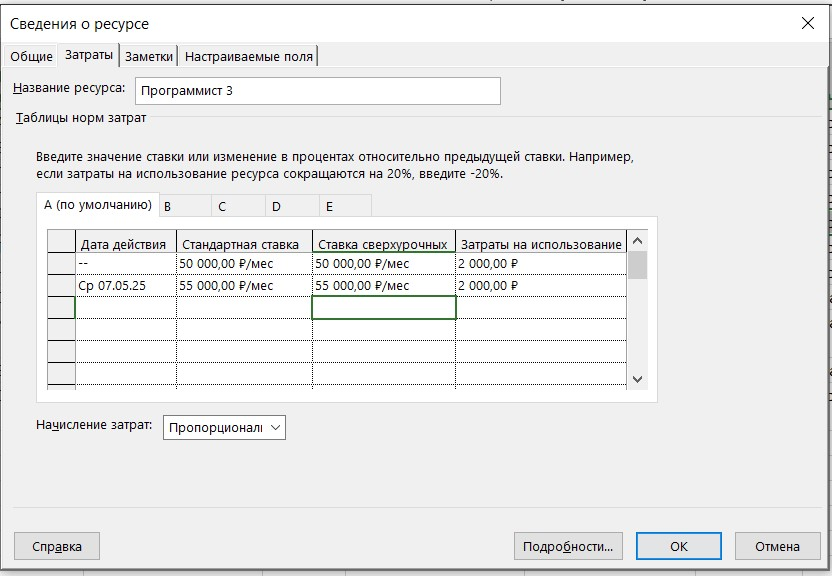
\includegraphics[width=0.9\textwidth]{img/task10/screen10_4.jpg}
	\caption{Обновление ставки программиста №3}
	\label{fig:screen10_4}
\end{figure}

Задача <<Постановка задачи>> фактически длилась 7 дней.

\begin{figure}[H]
	\centering
	
\includegraphics[width=0.9\textwidth]{img/task10/screen10_5.jpg}
	\caption{Обновление фактической длительности постановки задачи}
	\label{fig:screen10_5}
\end{figure}

Заполнение базы данных фактически длилось 10 дней.

\begin{figure}[H]
	\centering
	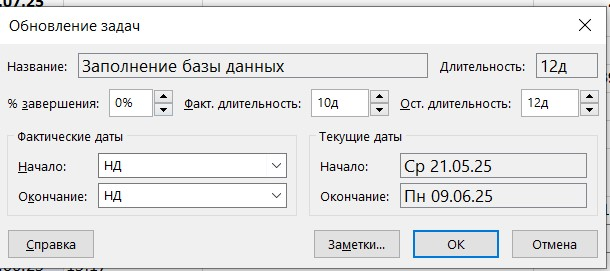
\includegraphics[width=0.9\textwidth]{img/task10/screen10_6.jpg}
	\caption{Обновление фактической длительности заполнения базы данных}
	\label{fig:screen10_6}
\end{figure}

Анализ отклонения от плана приведено на рисунке~\ref{fig:screen10_7}.

\begin{figure}[H]
	\centering
	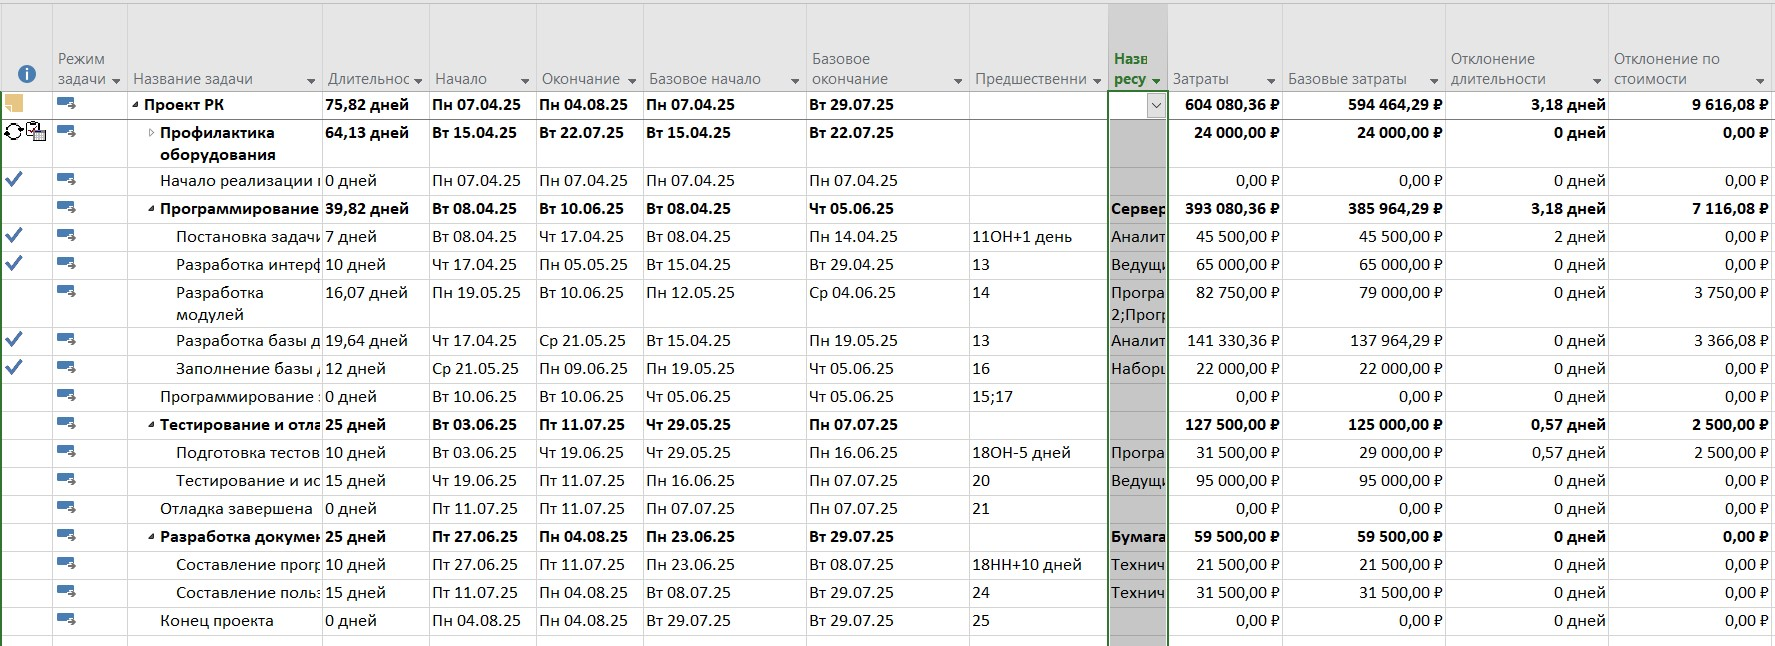
\includegraphics[width=0.9\textwidth]{img/task10/screen10_7.jpg}
	\caption{Отклонение от базового плана}
	\label{fig:screen10_7}
\end{figure}

Отклонение от базового плана по затратам составило 9616 рублей в большую сторону, отклонение длительности составило 3 дня, проект заканчивается 04.08 вместо 29.07.

Линия хода выполнения приведена на рисунке~\ref{fig:screen10_9}.

\begin{figure}[H]
	\centering
	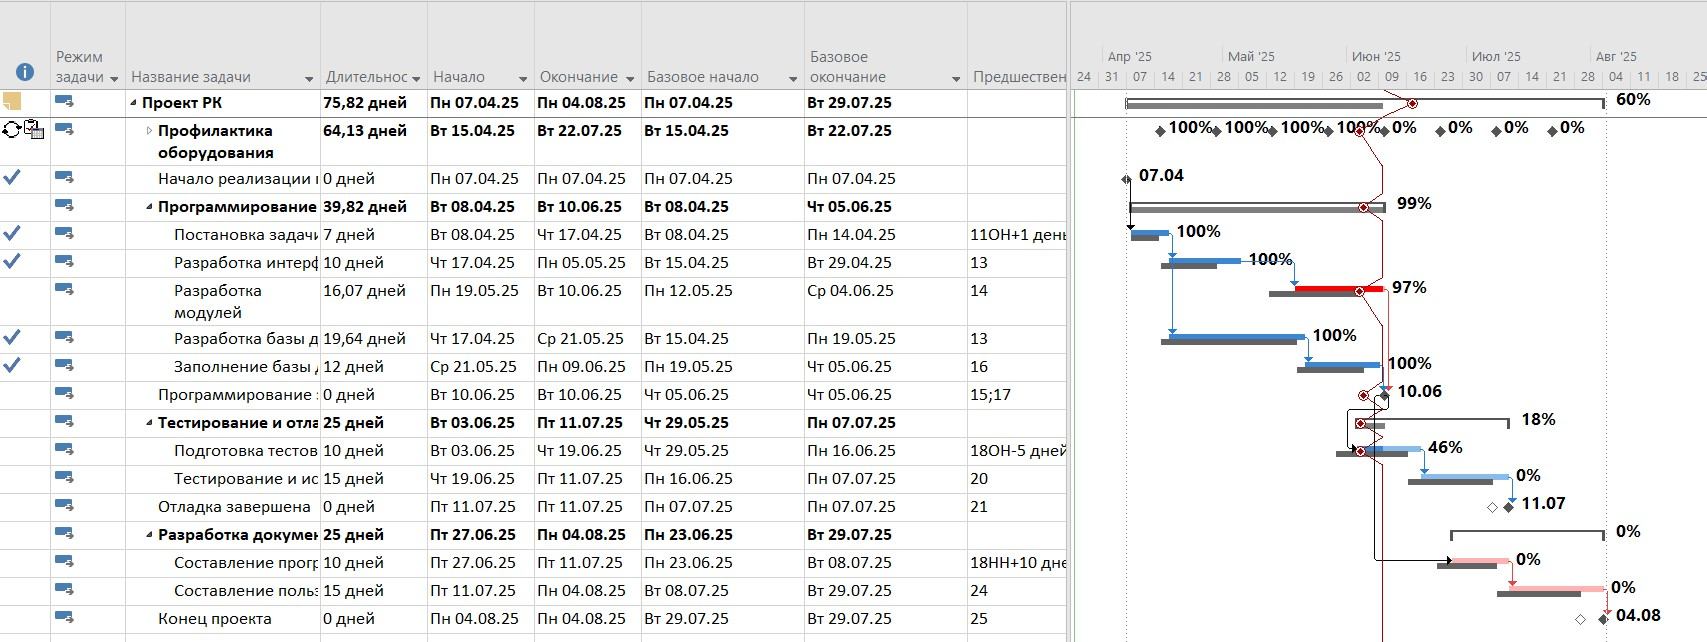
\includegraphics[width=0.9\textwidth]{img/task10/screen10_9.jpg}
	\caption{Линия хода выполнения}
	\label{fig:screen10_9}
\end{figure}

По отклонению линии хода выполнения влево можно сказать, что веха <<Программирование>>, а именно разработка модулей отстает от плана. Тестирование также отстает от плана из-за задержки задач по программированию.

Таблица освоенного объема приведена на рисунке~\ref{fig:screen10_10}.

\begin{figure}[H]
	\centering
	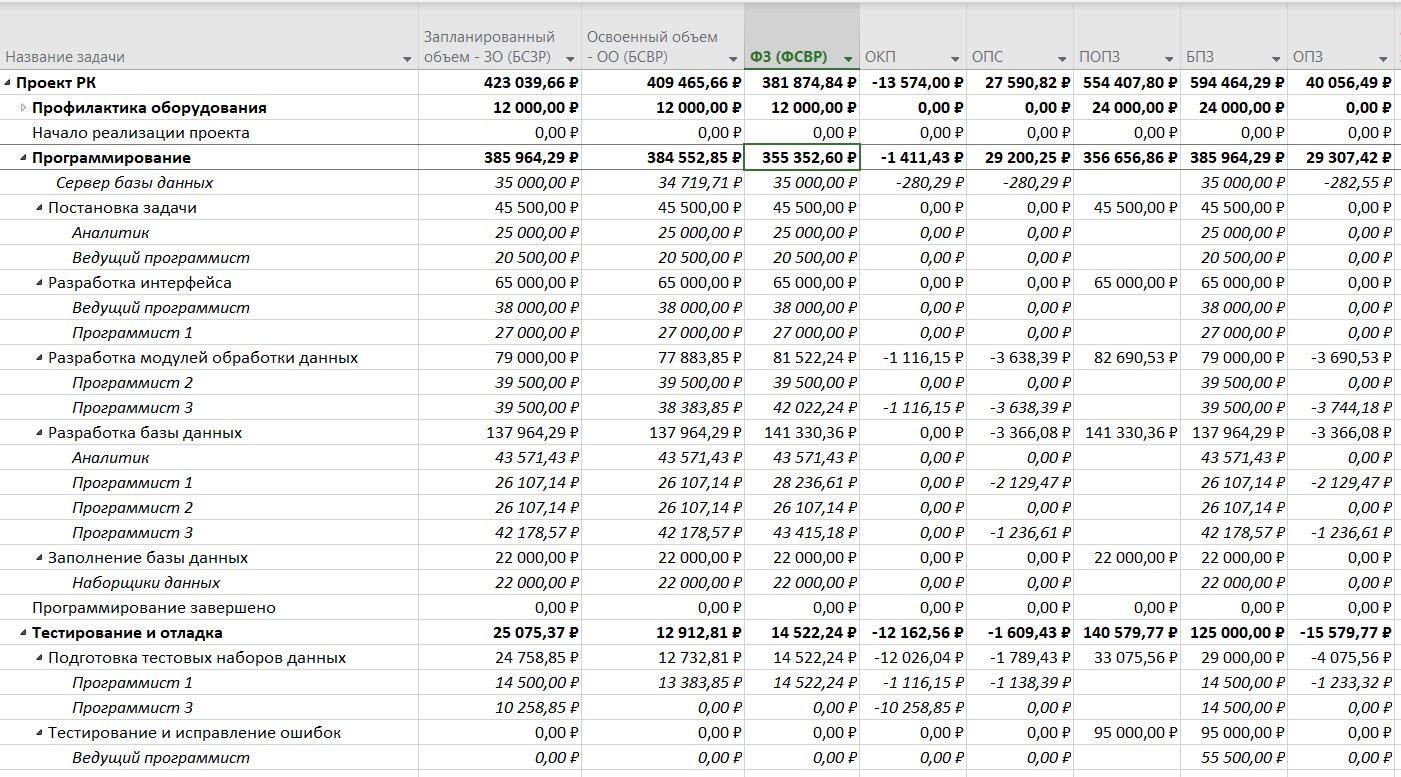
\includegraphics[width=0.9\textwidth]{img/task10/screen10_10.jpg}
	\caption{Таблица освоенного объема}
	\label{fig:screen10_10}
\end{figure}

ОКП $< 0$ из-за задержки задач <<Постановка задачи>> на 2 дня, что повлияло на задачу <<Разработка модулей обработки данных>>, которая завершается 10.06 вместо 05.06, тем самым являясь выполненной лишь на 97\% на момент отчета.
Также из-за задержки завершения задач по программированию, задачи тестирования начались позже (03.06 вместо 29.05), из-за чего задача <<Подготовка тестовых наборов данных>> выполнена в меньшем объеме, чем планировалось.

ОПС должен быть меньше нуля, если смотреть ОПС каждого отдельного ресурса по задаче $> 0$.
Проджект учитывает в ОО сервер, а в ФЗ не учитывает.
ОПС в задачах, где после 07.05 участвуют программисты 1 и 3 меньше нуля, так как их зарплаты выросли на 10\%. 


\section{Задание №11}

Проект укладывается в бюджет с запасом 20000 рублей, что не является достаточным запасом для проекта подобного масштаба.
Во временные сроки проект укладывается и заканчивается по базовому плану 29.07, а с учетом введенных изменений 04.08, что также не является достаточным запасом по времени.

